\documentclass[12pt,a4paper]{article}
\usepackage[utf8]{inputenc}
\usepackage{amsmath}
\usepackage{amsfonts}
\usepackage{amssymb}
\usepackage{tikz}
\usepackage{amsopn}
\usetikzlibrary{arrows}
\newtheorem{theorem}{Theorem}
\newtheorem{definition}{Definition}
\usepackage{standalone}
\usepackage{tikz}
\usepackage[ruled,vlined]{algorithm2e}
\usetikzlibrary{matrix,chains,positioning,decorations.pathreplacing,arrows}
\usetikzlibrary{positioning,calc}

\begin{document}
\bibliographystyle{plain}
\title{Neural Networks}
\maketitle

Neural Networks have the remarkable property that they are able to improve their performance with more data. In many other methods more data certainly helps, but the performance of the algorthms tends to achieve a plateau upon a certain amount of data. Furthermore nowadays more complex MM architectures can be run. So NN benefit from enhanced computer power because we are able to 1) handle more data 2)build more complex architectures, and 3) NN particularily benefit from more data. A summary of historic as well as recent developments and achievement of NN can be found in Ref. \cite{DBLP:journals/corr/Schmidhuber14}.

NN are typically used for supervised learning problem. They had quite some success for unstructured data (images, audio). So we can roughly say that there are the following main architectures:
\begin{itemize}	\setlength\itemsep{0em}
\item Standard NN (classification)
\item Convolutional NN (image data)
\item Recurrent NN (time series, sequence data)

\end{itemize}

\section{Notation} 
We start with the notation for a classification. Todo: generalize this
\begin{itemize}	\setlength\itemsep{0em}
\item $m$ Number of training examples
\item $x^i$ $i$-th feature, $x^i \in \mathbb R ^ {n_x}$ 
\item with $n_x$ the number of features
\item $y^i$ $i$-th label, $y^i \in \mathcal Y$
\item $\tilde y^i$ $i$-th predicted label $\tilde y^i \in \mathcal Y$
\item with $\mathcal Y$ the individual target classes.
\item Feature Matrix $\mathbb R^{m \times n_x} \ni M = \left(x^1, \dots x^m\right)  $ 
\item Label vector $\mathbb R ^m \ni Y    = (y^1, \dots y^m)$
\end{itemize}
So the columns of the feature Matrix are the individual training features. Note that in other frameworks the feature matrix is defined as the transpose

\section{Activation Functions}
\paragraph{Non-linear activation functions}
\begin{itemize}
\item Sigmoid function
\begin{align}
	f(x) = \frac{1}{1+e^{-x}}
\end{align}
\item tanh activation function
\begin{align}
	f(x)=\tanh(x)
\end{align}
\item Rectified linear unit (Relu)
\begin{align}
f (x) = \left\{
\begin{array}{ll}
x & x \geq 0 \\
0 &  x < 0  \\
\end{array}
\right. 
\end{align}
\item Leaky Relu
\begin{align}
f (x) = \left\{
\begin{array}{ll}
x & x \geq 0 \\
\alpha x &  x < 0  \\
\end{array}
\right. ~ \alpha \geq 0
\end{align}
\end{itemize}
In practice the sigmoid function is not used, except for output layers in classification tasks.
The tanh function outperforms the sigmoid function, since it symmetrizes the sigmoid function and thus has mean of zero. 
Currently the gold standard is the Relu function, which ameliorates problems with very small derives of the tanh activation function. Since the Relu function is $0$ for $z<0$ and thus gives zero derivatives, the leaky relu function avoids this by setting a very small constant negatve slope for $z<0$. In practice there does not seem to be much of a difference between relu and leaky relu.  

Note that all these activation functions are non-linear.

\paragraph{Non-linear activation functions}
In principle there are also linear activation $a=Mz +b$ functions thinkable. These include the identity function. However note, that these destroy the advantage of hidden layers because the linear combination of linear functions is linear. The only useful usecase is to use e.g. the identity activation in the output layer in a regression problem. 

\paragraph{Output-layer activation functions}
Typically in a deep neural network the Relu activation function is used. Only the output layer plays a special role as it needs to reflect the problem structure. 
\begin{itemize}	\setlength\itemsep{0em}
	\item Binary classification 
	\item Multi-class classification
\end{itemize}

\section{Loss and cost functions}
\begin{definition}[Loss function] Let there be the true label $y \in \mathcal Y$ and the predicted label $\tilde y \in \mathcal Y$ for feature x.
Then a loss function is a map
\begin{align*}
L: \mathcal Y \times \mathcal Y \rightarrow \mathbb R
\end{align*}
\end{definition}
Note that the loss function depends on the problem at hand and should be defined appropriately.
\begin{definition}[Cost function] 
\begin{align*}
J = \frac{1}{m}\sum_{i=1} ^m L (y^i, \tilde{y}^i)  
\end{align*} 
\end{definition}

\paragraph*{Examples}
\begin{itemize}
\item Quadratic loss function: $L(y, \tilde y) = \frac{1}{2}(y-\tilde{y})^2$
\item Logistic regression loss function: $L(y, \tilde y) = - y\ln \tilde y - (1-y)\ln (1 - \tilde y)$
\end{itemize}
Eventually the cost function needs to be minimized. Numerically this is done by using optimizers such as gradient descent. However, these are local optimizers and a \textbf{convex} loss function is essential in order to find the global optimum.

\paragraph*{Logistic regression}
The Logistic Regression is given
\begin{align}
\tilde y &= \sigma(w^T x + b) \\
\sigma(z) &= \frac{1}{1+e^{-x}}, 
\end{align}
where $\sigma$ is the logist function, $x$ the training features, and $w$ the model parameters to be learned. $\tilde y$ is interpreted as the probability of beeing in class 1 (and $1 - \tilde y$ as the probability of beeing in class 0). Summarizing, we get
\begin{align}
p(y=1 | x) &= \tilde y \\
p(y=0 | x) &= 1 - \tilde y,
\end{align} 
which can be expressed more compactly as
\begin{align}
p(y|x) = \tilde y ^y (1-\tilde y)^{1-y}
\end{align}
Taking the negative logartithm of this expression just gives the logistic regression loss function. The negative because just the logarithm would yield an objective function to be maximised and the loss function is a quantity we would like to minimize. The associated cost function may be obtained by assuming iid of training data. The total probability then $p(\{y_n\}|\{x_n\}) = \prod_n p(y_n|x_n)$. Using the same argument as for the loss function gives the logistic cost function.
\section{Predicting and training}
Once a NN is specified (architecture, definition of units and activation functions), it needs to be trained and eventually used to compute predictions. A NN may be understood as a computational graph. Together with the the concepts of forward and backward propagation training and predicting is done on this computational graph. 
\paragraph{Predicting.}
Forward propagation is used to compute the output of the NN and thus is equivalent to the prediction step.
\paragraph{Training.} Backward propagation is used to compute the gradients. This is the basic ingredient for computing the parameters of a NN, i.e. the training step. This is achieved by minimizing the cost function. Once the gradients are computed by back propagation algorithm \cite{Rumelhart:backpropagation} of the NN corresponds to minimizing the cost function with respect to the parameter space of the NN.
As in the specification step of the NN the gradients need to be computed individually.

\paragraph{Gradient descent.} Gradient descent is a common method to train the NN. Note that the parameters should be \textbf{initialized  randomly} in order to achieve symmetry breaking. Furthermore for these parameters should be chosen to be small in order to avoid too small gradients, which eventually results in slow learning. Strictly speaking this only holds true for activation functions such as the sigmoid or tanh, which exhibit very small gradients for large input values (that is why we want to keep the input values small upon initialization). 

\section{Deep neural Networks}
Deep neural networks have several hidden layers (Figure \ref{fig:deep_neural_net}). The intuition behind this is, that the first layer finds very local details of the input (simple functions of the input). The ensuing layers then add more complex representations of the overall output (compositional representation).
\begin{figure}
	%\includestandalone[width=\textwidth]{deep_net_diagramm}
	\documentclass{standalone}
\usepackage{tikz}
\usetikzlibrary{matrix,chains,positioning,decorations.pathreplacing,arrows}
\usetikzlibrary{positioning,calc}
\begin{document}

\tikzset{%
  every neuron/.style={
    circle,
    draw,
    minimum size=1cm
  },
  neuron missing/.style={
    draw=none, 
    scale=4,
    text height=0.333cm,
    execute at begin node=\color{black}$\vdots$
  },
}

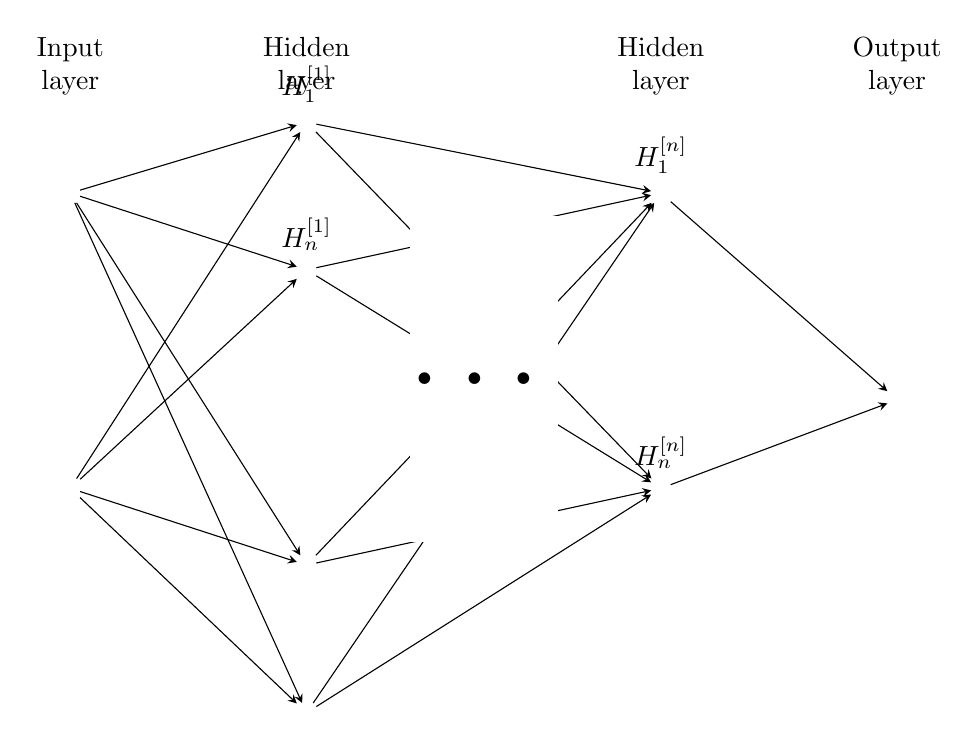
\begin{tikzpicture}[x=1.5cm, y=1.5cm, >=stealth]

\foreach \m/\l [count=\y] in {1,missing,2}
  \node [every neuron/.try, neuron \m/.try] (input-\m) at (0,2.5-\y*1.25) {};

\foreach \m [count=\y] in {1,2,missing,3,4}
  \node [every neuron/.try, neuron \m/.try ] (hidden1-\m) at (2,3.1-\y*1.25) {};

%\foreach \m [count=\y] in {1,missing,2}
%\node [every neuron/.try, neuron \m/.try ] (hidden1-\m) at (2,2-\y*1.25) {};

\foreach \m [count=\y] in {1,missing,2}
  \node [every neuron/.try, neuron \m/.try ] (hidden2-\m) at (5,2.5-\y*1.25) {};

\foreach \m [count=\y] in {1}
  \node [every neuron/.try, neuron \m/.try ] (output-\m) at (7,.5-\y) {};

% arrows to input labels
%\foreach \l [count=\i] in {1,2,3,n}
%  \draw [<-] (input-\i) -- ++(-1,0)
%    node [above, midway] {$I_\l$};

\foreach \l [count=\i] in {1,n}
  \node [above] at (hidden1-\i.north) {$H^{[1]}_\l$};

\foreach \l [count=\i] in {1,n}
  \node [above] at (hidden2-\i.north) {$H^{[n]}_\l$};

% arrows on output label
%\foreach \l [count=\i] in {1}
%  \draw [->] (output-\i) -- ++(1,0)
%    node [above, midway] {$O_\l$};


\foreach \i in {1,...,2}
  \foreach \j in {1,...,4}
    \draw [->] (input-\i) -- (hidden1-\j);

\foreach \i in {1,...,4}
  \foreach \j in {1,...,2}
    \draw [->] (hidden1-\i) -- (hidden2-\j);

    \foreach \i in {1,...,2}
    \foreach \j in {1}
    \draw [->] (hidden2-\i) -- (output-\j);

\node [align=center, above] at (0,2) {Input\\layer};
\node [align=center, above] at (2,2) {Hidden \\layer};
\node [align=center, above] at (5,2) {Hidden \\layer};
\node [align=center, above] at (7,2) {Output \\layer};

% lonsome dots
\node[fill=white,scale=4,inner xsep=0pt,inner ysep=5mm] at ($(hidden1-2)!.5!(hidden2-2)$) {$\dots$};

\end{tikzpicture}
\end{document}
	\caption{Illustration of a  deep neural network with a single output unit.}
	\label{fig:deep_neural_net}
\end{figure}
There are several motivations behind such a layered architecture:
\begin{itemize} 
\item Universal approximation theorem 	
\item Circuit theory: one may compute functions with a small (i.e., not many hidden units per layer) deep neural network that would require exponentially many hidden units in a shallow NN \cite{2014arXiv1402.1869M}. The infamous example is computing XOR on (all) the features (note that XOR itself with AND and OR functions itself already needs a deep neural network).
\item An exhausitve list of arguments can be found in \cite{Goodfellow:2016:DL} Chap 6.4

\end{itemize}
\paragraph{Definition and Conventions}
\begin{itemize}	\setlength\itemsep{0em}
	\item $W^{[l]}, b^{[l]}$: Weights of layer $l$
	\item $g^{[l]}$: Activation function of layer $l$
	\item $n^{[l]}$: Number of units in layer $l$
\end{itemize}
Note that the structure depicted in the graphical representation refers to a \textbf{single} training example. In implementations we usually work with vectorized formulars.
\paragraph{Parameters vs Hyperparameters.} Parameters are just the weights $W^{[l]}, b^{[l]}$. These are the quantity to be trained. All other quantities (Number of layers $l$, number of units in layer $l$, activation function of layer $l$, learning rate, ...) are called Hyperparameters.  These quantities must be set empirically.
\paragraph{Forward and Backpropagation}
\paragraph{Vectorized version}
\paragraph{Initialization}

\section{Optimizing Neural Networks}
The predictive performance  of a neureal network depends on the hyperparameters and its architecture. First the necessary concepts for judging the predictive power are presented. Based on that, concepts to improve the prediction accuracy are summarized.
\subsection{Train, development and test set.}
It's common practice to split the Data in 3 Sets: Training set, Hold-out crossvalidation (or development) set, and Test set. The Training set is used to train the model. The development set is used to test specific models and based on that develop better models. Once the choice for the best model is made the test set is used to get an \emph{unbiased} estimate of the model performance. If no unbiased estimate on the model is needed sometimes only train and dev sets are used. How to split the data depends on the amount of data:
\begin{itemize}
	\item \textbf{Conventionally} the splitting was made in the order of $70\,\%  - 30 \,\%$  (omitting the test set) or $60\,\% - 20 \,\% - 20\,\%$. This applies $\approx 10^5$ datapoints on order to make sure to have enough test examples.
	\item \textbf{Big data} usecases with $> 10^6$ datapoints typically have splittings in the order $98\,\% - 1 \,\% - 1 \,\%$  because there are still enough samples for the test statistics.
\end{itemize}

Since neural networks need a lot of data some applications use mismatched data distributions between the training set and development and test distributions. E.g., the training data come from webcrawling and the develpment and test sets come from the specific application at hand. However, in this case it is necessary that the development and the test set come from the same distribution.

\subsection{Bias and Variance.}
The \textbf{bias} of a model describes the complexity of the model. A model with high bias has a (too) simple decision boundary (e.g., linear regression). The bias may be assessed by the model performance on the training set. The \textbf{variance} describes the generalization property of model. A model with high variance tends to perform worse for new data (development set). High variance is also called \textbf{over-fitting}.

An example is given in Table \ref{table:bias_variance}. The worst case is model M3 (high bias and high variance). The ideal case is model M4 (low bias and low variance). Note that the model assessment in Table \ref{table:bias_variance} is based on the assumption that the true labeling contained in train and development set are known without error (the Bayesian error is 0\,\%).  A counterexample to this assumption would be blurry images, where even humans make errors in labeling. 
\begin{table}[]\label{table:bias_variance}

	\begin{tabular}{l llll}
		\hline   \hline
		 model &M1 &M2 &M3 &M4 \\
		\hline 
		Training set error [\%]  &1  &15  &15  &0.5 \\
		Development set  error  [\%]       &11 &16  &30  &1 \\
		\hline
		Problem diagnosis	& high variance &  high bias & high bias & low bias \\
							&  &  & high variance & low variance \\
							\hline \hline					 
	\end{tabular}
\caption{Illustration of bias and variance for 4 models M1 ... M4. .}
\end{table}
Bias and variance  are important quantities upon improving the model performance:
\paragraph{Strategies to reduce bias:}
\begin{itemize}
	\setlength\itemsep{0em}
	\item Bigger network (number of layers / units / hyperparameter search) 
	\item Train longer 
	\item Use other optimization algorithm
	\item Different NN architecture
\end{itemize}
\paragraph{Strategies to reduce variance:}
\begin{itemize}
	\setlength\itemsep{0em}
	\item More training data
	\item Regularization
	\item Different NN architecture
\end{itemize}
By iteration through bias reduction and variance reduction one can systematically improve the model performance. Note that in the case of neural networks reducing the bias and reducing the variance can be done relatively independently. This is a further advantage of neural networks. In the 'old days' one needed to find a bias variance trade off as these two quantities could not be improved independently. Probably the main reason is that nowadays there are much more data at hand. Also note that regularization also affects the bias.

The purpose of the test set is to judge the final performance of the algorithm. Ideally development set and test set error are very similar. However, if the test set error is much larger than the training set error then the development set should be increased.

\subsection{Regularization}
Regularization aims to reduce the variance, i.e., reduce generalization errors. There are several regularization strategies for neural networks \cite{Srihari:regularization_talk, Goodfellow:2016:DL}:	

\paragraph{Parameter norm penalties.} This procedure is also called weight decay and follows the same ideas as standard regularization.  Then this regularization scheme adds to the cost function $J(\theta)$  a penalty term
\begin{align}
    \tilde J(\theta)  =  J(\theta) + \lambda \Omega(\theta), 
%	J \mapsto J - \frac{\lambda}{2m} \sum _{l=1}^L \lVert w^{[l]} \rVert _F ^2, 
\end{align}
where $\lambda$ is an additional hyperparameter and $\theta$ are model parameters, which are determined by minimizing the cost function. $\tilde J$ is then used instead of $J$ as objective function in order to determine the modelparmeters within an optimization algorithm. 
In the specific case of a deep neural network a common regularization scheme is
\begin{align}
	\tilde J(\{w^{[l]}, b^{[l]}\}) =  J(\{w^{[l]}, b^{[l]}\}) + \frac{\lambda}{2m} \sum _{i=1}^L \lVert w^{[i]} \rVert _F ^2, 
\end{align}
where $w^{[l]}, b^{[l]}$ are the weights of layer $l$, $\lVert w \rVert _F$ is the Frobenius norm  ($\lVert w \rVert _F ^2 = \sum_{i, j} w_{ij}^2$,) and $m$ is the number of training examples. This procedure is also called weight decay. Note that in this scheme only the $w^{[l]}$ are regularized - probably because there are much more parameters than in the $b^{[l]}$ and the assumption that this leads to a sufficient regularization.

\textit{Remark:} The disadvantage of this approach is the scaling properties are lost. These can be recovered by regularizing not all layers \cite{Srihari:regularization_talk} ?!?	

\paragraph{Dropout.} In dropout regularization nodes and its edges are removed at random for each training example. This introduces a new hyperparamter the "survival" probability of a node.  This probability can be layer dependent. In particular layers with many units that are suspicious to overfitting may be assigned lower survival probabilities than layers with only a few units. In principle dropout can be also used in the input layer. Dropout has been successful in particular in computer vision. Dropout is implemented by masking the activation with a boolean random draw of of a Bernoulli experiment with given survival probability. In practice  "inverse dropout" is used, which additionally divides the activations by the the survival probability.

\textit{Remark:} With dropout the cost function $J$ is no longer well defined. So the convergence behaviour of $J$ as monotonically decreasing function during iteration is lost.

\paragraph{Data augmentation.} Reduces the variance by artificially creating more data via e.g., random rotations, distortions, flips, crops of images. This approach does \textit{not} introduce new hyper parameters.

\paragraph{Early stopping.} This approach tries to reduce over fitting by "tweaking"  the optimization step. Instead of ensuring, that the cost function w.r.t to the training data is minimized, additionally the cost function or error w.r.t the development set is monitored (optimization is still performed with the training set). One then stops at the optimization step where the cost function of the development data is minimized. This approach roots in the observation, that typically the development set error decreases with increasing optimization steps but then starts to increase again. This approach does \textit{not} introduce new hyperparameters.

\paragraph{Further regularization techniques\cite{Srihari:regularization_talk}:}
\begin{itemize}
	\setlength\itemsep{0em}
	\item Parameter tying and sharing
	\item Bagging/ensemble methods
	\item Tangent methods
	\item Adversarial training
\end{itemize}

\section{Optimization algorithms} \label{sec:optimizers}
Given an objective function $J(\theta)$ an optimization algorithm tries to find a local minimizer $\theta ^* = \operatorname{argmin}_\theta J(\theta)$ \cite{NoceWrig06}. To this end an optimization algorithm generates a sequence of iterates $\{\theta_k\}_{k=0} ^\infty$ that (ideally) terminate at the minimizer. Different algorithms differ the process of generating these iterates. $\theta_0$ is often called initialization. For brevity we will use the notation $\nabla J_k \equiv \nabla_\theta J(\theta)\rvert_{\theta_k}$.   
\subsection{Algorithms used for neural networks}
\paragraph{Gradient descent.}
The update in gradient descent is given by
\begin{align} \label{eq:gradient_descent}
	\theta_{k+1} = \theta_k - \alpha \nabla J_k,
\end{align}
where $\alpha$ is called learning rate (hyper parameter).

\paragraph{Exponentially moving average (EMA).} This is not an optimization algorithm itself but a very common ingredient. Exponentially moving average is a comutationally efficient method to approximate moving averages.
Gradient descent may produce oscillating gradients, which induce a reduced learning rate in order to achieve convergence. Many alogrithmic improvements of gradient descent are based on the first and second moment of the gradient. 

For example, in order to soften  oscillations one could use the moving average over the last $m$ computed derivatives, $\bar \nabla J_k := 1/m \sum_{i=k-m} ^ k \nabla J_k$ instead of the current gradient in Equation \ref{eq:gradient_descent}. However, this would require storing $m-1$ additional gradients. Instead,  the moments are approximated by the exponentially moving average.

Assume a series of data $\{q_k\}$. Then the exponentially moving average is defined iteratively as
\begin{align}
\langle  q \rangle ^{\text{EMA}}_0 &= 0\\ 
\langle  q \rangle ^{\text{EMA}}_k &= \frac{1}{1-\beta^k}\left(\beta \langle  q \rangle ^{\text{EMA}}_{k-1}+ (1-\beta) q_k\right) \label{eq:ema}
\end{align}
There is also refined version of exponentially moving average  that includes bias correction,
\begin{align}
\langle  q \rangle ^{\text{cEMA}}_0 &= 0\\ 
\langle  q \rangle ^{\text{cEMA}}_k &= \frac{1}{1-\beta^k}\left(\beta \langle  q \rangle ^{\text{EMA}}_{k-1}+ (1-\beta) q_k\right)
\end{align}

The term $1/\left(1-\beta^k\right)$ is called \textit{bias correction}. It corrects  detoriations for the first few data points.

\paragraph{Gradient descent with momentum.} 
Gradient descent with momentum replaces the gradient by its first moment (expectation value) obtained by the exponentially weighted average \ref{eq:ema}. The update procedure of \ref{eq:gradient_descent} gets then modified to:
\begin{align}
	 \langle  \nabla J \rangle ^{\text{EMA}}_0 &= 0  ~ \text{(initialization)} \\ 
	\langle  \nabla J \rangle ^{\text{EMA}}_k &= \beta \langle  \nabla J \rangle ^{\text{EMA}}_{k-1}+ (1-\beta) \nabla J_k \\
	\theta_{k+1} &= \theta_k - \alpha 	\langle  \nabla J \rangle ^{\text{EMA}}_k. \label{eq:gradient_moments_update}
\end{align}
The term $\langle  \nabla J \rangle ^{\text{EMA}}_{k-1}$ is called momentum, which lends the algorithm it's name.
$\beta$ describes how many past gradients are used and is in principle an other hyper parameter. In practice it is often set to $\beta=0.8$. Gradient descent with momentum converge typically  faster than gradient descent.

\paragraph{RMSprop \cite{Tieleman2012}.} Gradient descent with momentum damps gradient oscillations by using the approximate averages over the previous gradients. RMSprop  ("Root mean square propagation") tries to damp oscillation in a complementary fashion. It weights the gradient by the inverse of the root mean square of the previous gradients  -- again using as exponentially moving averages as approximations to the average. 

\begin{align}
	\langle \nabla J  \odot \nabla J\rangle ^{\text{EMA}}_0 &= 0   ~ \text{(initialization)}\\ 
		\langle \nabla J  \odot \nabla J\rangle^{\text{EMA}}_k &= \beta \langle \nabla J  \odot \nabla J\rangle^{\text{EMA}}_{k -1} + (1-\beta) \nabla J_k  \odot \nabla J_k, \\
	   \theta_{k+1} &= \theta_k - \alpha \nabla J_k \oslash \left(\sqrt{\langle \nabla J  \odot \nabla J\rangle^{\text{EMA}}_k} + \epsilon \right), \label{eq:rms_prop_update} 
\end{align} 
where the square rood is taken elementwise $(\sqrt{A})_{ij} = \sqrt{A_{ij}}$, and  the  elementwise
 (Hadamard) product $\left(A\odot B\right)_{ij} = A_{ij} B_{ij}$ and division  $\left(A\oslash B\right)_{ij} = A_{ij} / B_{ij}$ is used. The matrix $\epsilon$ prevents division by zero and it's components are typically set to $10^{-8}$. The expression $\langle \nabla J  \odot \nabla J\rangle^{\text{EMA}}_k$ is the element wise second moment of the gradient within the EMA approximation. Thus, the RMSprop update \ref{eq:rms_prop_update} scales the gradients by the element wise RMS (root mean square) using EMA. As with gradient descent with momentum, $\beta$ introduces a new hyper paramter but it's typically set to $\beta=0.8$.

\paragraph{Adam \cite{AdamOptimizer2014}.} Adaptive moment estimation (Adam) combines gradient descent with momentum with RMSprop. It takes the averaged gradients as in \ref{eq:gradient_moments_update} and scales them according to RMSprop \ref{eq:rms_prop_update}. However, instead of using EMA the bias corrected EMA is used. Adam then updates the optimization steps according to
\begin{itemize}	\setlength\itemsep{0em}
	\item Initialize $\theta$ and first and second moments of gradients
	\begin{align*}
	\langle  \nabla J \rangle ^{\text{cEMA}}_0 &= 0   \\ 
	\langle \nabla J  \odot \nabla J\rangle ^{\text{cEMA}}_0 &= 0  
	\end{align*}
	\item Update Update moments
	\begin{align*}
	\langle  \nabla J \rangle ^{\text{cEMA}}_k &= \frac{1}{1-\beta_1^k}\left( \beta_1 \langle  \nabla J \rangle ^{\text{EMA}}_{k-1}+ (1-\beta_1) \nabla J_k \right)\\
	\langle \nabla J  \odot \nabla J\rangle^{\text{cEMA}}_k &= \frac{1}{1-\beta_2^k}\left( \beta_2 \langle \nabla J  \odot \nabla J\rangle^{\text{EMA}}_{k -1} + (1-\beta_2) \nabla J_k  \odot \nabla J_k\right) 
	\end{align*}
	\item Update optimization step
	\begin{align}
	\theta_{k+1} = \theta_k - \alpha \langle  \nabla J \rangle ^{\text{cEMA}}_k \oslash \left(\sqrt{\langle \nabla J  \odot \nabla J\rangle^{\text{cEMA}}_k} + \epsilon \right), \label{eq:adam_update} 
	\end{align}
\end{itemize}
Apart from the learning rate $\alpha$ there are in principle three additional hyper parameters: $\beta_1, \beta_2, \epsilon$. In practice these are not tuned but set to the values $\beta_1 = 0.9, \beta_2=0.999, \epsilon=10^{-8}$ \cite{AdamOptimizer2014}.

\subsection{Problems of optimizers for neural networks}
We briefly judge the optimization strategies for neural networks
\begin{itemize}\setlength\itemsep{0em}
	\item Neural networks pose a \textbf{non-convex optimization problem}. However, the algorithms above are modifications of established algorithms for convex optimization problems. So it would be desirable to have non-convex optimization algorithms.
	\item In principle neural networks may have \textbf{many local minima} and the optimization algorithm finds one of them (of course one would like to find the global minimum). This problem has been debated intensively in the community. However, there is an interesting counterargument: in order to have a local minimum $\theta^*$ \textit{all} components of the second derivative at the minimum must be greater than zero $\partial_\theta ^2 J \rvert _{\theta^*} > 0$. Howver, for a very large NN where $\theta$ is high dimensional (several thousand components) this is very unlikely. So extremal points are most probably saddle points, which don't pose a problem to the the above optimizers. This is a consequence, that low dimensional intuition does not necessarily carry over to high dimensional neural networks.
	\item \textbf{Flat regions} of the cost functions may lead to very slow learning. Algorithms like Adam tend to reduce this problem, but it can still be severe.
	\item All algorithms of section  \ref{sec:optimizers} only use the first derivative of the cost function (and it's first and / or second moments). However in the literature the most powerful standard algorithms also use the second derivative (\textbf{Hessian}).
	\item Mind the paradigm: "In practice, it is more important to choose a model family that is easy to optimize than to use a powerful optimization algorithm" \cite{Goodfellow:2016:DL}. 
\end{itemize}
In summary, there seems to be quite some room for improving optimization algorithms \cite{2017arXiv170807827X}. 


\subsection{Speed up the learning process}
Training a NN is optimizing the cost function with respect ot the parameters. In practice this can be a tricky task for several reasons:
\begin{itemize}\setlength\itemsep{0em}
	\item Algorithm specific problems: learning rate
	\item NN architecture specific problems: vanishing or exploding gradients for (very) deep neural networks.
	\item Large training data (slow computations).
\end{itemize}
For these reasons optimization in neural networks is yet not well understood. We summerize some heuristics often used in the community.

\paragraph{Data normalization.} When data are in the same numerical range a larger learning rate can be chosen. 
\paragraph{Weight initialization.} The problem of vanishing or exploding gradients can be partially reduced by carefully initializing the weights. The weights are initialized by drawing from samples from the unit normal distribution, $\mathcal N(1,0)$ followed by a calibration transformation. The latter depends on the activation function but it's main rational is to account for different number of nodes per layer via a variance argument. Popular initialization schemes are:
\begin{itemize}\setlength\itemsep{0em}
	\item Reilu activation: $w^{[l]}_{ij} = \mathcal N(1,0) \sqrt{\frac{2}{n^{[l-1]}}}$
	\item Tanh activation: $w^{[l]}_{ij} = \mathcal N(1,0) \sqrt{\frac{1}{n^{[l-1]}}}$ (Xavier initialization),
\end{itemize}
where $n^{[l-1]}$ is the number of nodes in layer $n-1$. The aim of these initialization schemes is to reduce the tendency of gradients to explode or vanish for very deep neural networks.

\paragraph{Mini-batch gradient descent.} For moderately many training data a vectorized implementation of gradient descent may have an acceptable speed. In this version all training examples are passed into a single optimization step, which is also called batch (gradient descent). However, for many training examples  (larger than $\sim 10^3$) this may become slow. Mini-batch gradient descent splits the data in mini batches of size. Each optimization step then only sees one mini batch (including the labels and cost function).

An \textbf{epoch} is an entire pass through the training set. While batch gradient descent allows only one optimization step per epoch, mini-batch gradient descent allows for batch size over mini-batch size many optimization steps in one epoch. 

The extreme case of mini-batch size one is called \textbf{stochastic gradient descent}. The mini-batch size is another hyper parameter -- in practice typical values are powers of two in the range 64, 128, ... 512.

\paragraph{Learning rate decay} The algorithms in section  \ref{sec:optimizers} use a fixed learning rage $\alpha$. Intuitively, near the optimum the learning rate should be smaller and larger at areas far away from the optimum. There are several heuristics that adapt the learning rate in terms of epochs $n_e$
\begin{itemize}\setlength\itemsep{0em}
	 \item 
	 	  $ \alpha = \frac{\alpha_0}{1+ d n_e}, $ with hyper parameters $\alpha_0$ (initial learning rate) and $d$ (decay rate).
	 \item $ \alpha = \alpha_0\,0.95^{n_e}, $ with hyper parameters $\alpha_0$ (initial learning rate).
	 \item  $ \alpha = \frac{\alpha_0\,d}{\sqrt{n_e}}, $ with hyper parameters with hyper parameters $\alpha_0$ (initial learning rate) and $d$.
	 	  
\end{itemize} 


\section{Convolutional neural networks}
Convolutional neural networks come from computer vision (image classification, object detection, neural style transfer, ...). If a forward deep neural network was used for such tasks it would yield a very high dimensional input space and thus parameter space. As a consequence, there would not be enough data to prevent overfitting\footnote{For example a $1000\times 1000$ pixel input image with 1000 units in the first hidden layer would lead to a $3\cdot10^6 \times 1000$ dimensional weight matrix just for the first hidden layer (the factor of 3 comes from the 3 RGB channels).}. 

\paragraph{Continuous case. }
Let $f, g: \mathbb R ^n \rightarrow \mathbb C$, then 
\begin{align}
	(f * g)(t) &= \int f(t') g(t - t') \, dt'  \quad \text{(\textbf{convolution})}\\
	(f \star g)(t) &= \int \overline {f(t')} g(t + t') \, dt' \quad \text{(\textbf{cross correlation})},
\end{align}
While these quantities look innocently similar the interpretation is different. Cross correlation is interpreted as the similarity of the functions $f$ and $g$ (shifted by $t$). As special case, the \textit{auto correlation} at lag $\tau$ is just the cross correlation with itself $R_f(\tau) = (f \star f)(\tau)$.  Convolution is interpreted as $f$ being  "smeared out" by a  $g$: $(f*g)(t)$ is the weighted "mean" of $f(t')$ by a function $g(t-t')$. The convolution satisfies the following properties:
\begin{itemize}
	\item Commutative $f*g = g* f$
	\item Associative 
	\item Distributive
	\item Identity $f * \delta = f$. And therefore the inverse convolution (if exisits) is defined as 
	\item Translational equivariance. $\tau_x(f*g) = (\tau_x f) * g =   f *  (\tau_x g)$, with the translation operator $(\tau_x(f))(y) = f(y-x)$ (convolution commutes with translation).
	
\end{itemize}

Introducing the mirror operater $Pf(t) = f(-t)$ these convolution and cross correlation are related by \footnote{Because $\overline{Pf} * g = \int \overline{f(-t')} g(t - t') \, dt' = \int \overline{f(t')} g(t + t') \, dt' = f \star g $}
\begin{align} \label{eq:relation_conv_corr_cont}
f \star g = \overline{Pf} * g.
\end{align}
So, if $f$ is hermitian (symmetric for real valued functions), $\overline {f}(t) = f(-t)$, then $f \star g = f * g$. And if both, $f$ and  $g$ are hermitian then the cross correlation is commutative, $f\star g = g \star f$. Convolution and Cross correlation is translational equivariant.

In practice, these quantities are often calculated using the convolution theorem. Consider the Fourier transform of a function $f \in L^1(\mathbb R ^n) $
\begin{align}
	 (\mathcal F f)(y) &= \frac{1}{\sqrt{2\pi}^n } \int f(x) e^{-iy\cdot x}\, dx \\
	 (\mathcal F^{-1} \hat f)(x) &= \frac{1}{\sqrt{2\pi}^n } \int \hat f(y) e^{iy\cdot x}\, dy,
\end{align}
where $\mathcal F^{-1} $ is the inverse Fourier transform and $y\cdot x$ is the standard scalar product ($x, y \in \mathbb R ^n$). The \textit{convolution theorem} states that, 
\begin{align}
	f * g = \mathcal F^{-1} (\mathcal F f \cdot  \mathcal F g), \\
    f \star g = \mathcal F^{-1} (\overline{\mathcal F f} \cdot  \mathcal F g).
\end{align}
with the pointwise product  $(f_1 \cdot f_2)(x) = f_1(x) \, f_2(x) $. The expression follows from (\ref{eq:relation_conv_corr_cont}) and $\mathcal F\{\overline{Pf}\} = \overline{\mathcal F f}$. Thus, convolution and cross correlation may be computed from (inverse) Fourier transforms.


\paragraph{Discrete convolution.} Let $F: \mathbb{Z}^d \rightarrow \mathbb{R}$ be a discrete function. Let $\Omega_r = [-r, r]^d \cap \mathbb{Z}^d$ and $\omega: \Omega_r \rightarrow \mathbb{R}$ be a $(2r + 1)^d$ dimensional filter kernel. Then the discrete convolution operator $*$ is defined as \cite{yu2016multiscale, dumoulin2018guide}
\begin{align}
	(F * k)(p) = \sum_{s+t = p}F(s)\, \omega(t),
\end{align}
where in the context of neural networks $F$ is called input feature map and the convolution is called output feature map. The filter kernel size $(2r + 1)^d$  determines the size a given filter locally looks at the input feature map. For neural networks this is also called \textit{receptive field}.

For example, in image processing  there are well known edge detection filter kernels, 
\begin{align}
	\left[
	\begin{array}{rrr}
	1 & 0 & -1 \\ 
	0 & 0 & 0 \\
	-1 & 0 & 1 \\ 
	\end{array}\right],
	\quad
	\left[
	\begin{array}{rrr}
	0 & -1 & 0 \\ 
	-1 & 4 & -1 \\
	0 & -1 & 0 \\ 
	\end{array}\right],	
		\quad
	 \left[
	\begin{array}{rrr}
	-1 & -1 & -1 \\ 
	-1 & 8 & -1 \\
	-1 & -1 & -1 \\ 
	\end{array}\right].	
\end{align}

\paragraph{Deconvolution and transposed convolution}\cite{zeiler_deconvolution_nn_2010}
\paragraph{Dilated and causal convolutions}\cite{yu2016multiscale, chen2016semantic}

\paragraph{Convolutions in neural networks.} There are several tweaks in the application of convolutions to neural networks
\begin{itemize}
	\item Filters are learned by back propagation.
	\item Activation function and bias.
	\item Discrete correlation instead of convolution.
	\item Several Filters in parallel (filterbanks)
	\item Dimensions
	\item Padding and strides
	\item Pooling
\end{itemize}

- https://cs231n.github.io/convolutional-networks/

- https://arxiv.org/pdf/1511.07122.pdf 
- http://torch.ch/blog/2016/02/04/resnets.html
- https://cs231n.github.io/optimization-2/

\section{Sequence Models}
Sequence models are largely motivated from natural language processing but also find application in time series modeling \cite{DBLP:journals/corr/FlunkertSG17, lim2020time, NEURIPS2018_5cf68969, wang2019deep, lim2020recurrent}.

Recurrent neural nets suffer from vanishing / exploding gradient problem. Furthermore they are not easily capable of considering events in the long past.  Eventually they suffer from big memory requirement and need long training. One reason is that they use the last hidden state in the encoder step. Gated recurrent units (GRU) ans long-short-term-memory (LSTM) try to incorporate more information from the past by a more sophisticated activation unit. However, NLP tasks still suffer from the last hidden state approach in the encoder step. One could heuristically incorporate more hidden encoder states and pass them into the decoder. 

A more sound approach is the  attention mechanism\cite{bahdanau2016neural, luong2015effective}, which weights the hidden states and passes them into the decoder. Incorporating the attention mechanism also in the encoder step is called self-attention. This leads to the concept of transformers \cite{vaswani2017attention, illustratedtransformer} and state of the art  NLP models like BERT \cite{DBLP:journals/corr/abs-1810-04805}  or GPT2 \cite{radford2019language, illustratedgpt2}.

\subsection{Recurrent Neural Networks (RNN)}
In contrast to feed forward neural networks RNNs are \textit{in principle} capable of looking at the whole time sequence. The basic idea is that, RNN cells contain an internal memory state $h_t \in \mathbb R^{d_h}$  which acts as a compact summary of past information. At each time step the memory state is updated with new observations \cite{salehinejad2018recent, lim2020time}.
Furthermore,  RNNs are related to Bayesian filtering in discrete state Markov models \cite{lim2020recurrent, barber}.  
\begin{figure}
	\documentclass{standalone}
\usepackage{tikz}
\usetikzlibrary{matrix,chains,positioning,decorations.pathreplacing,arrows}
\usetikzlibrary{positioning, calc, chains}
\begin{document}


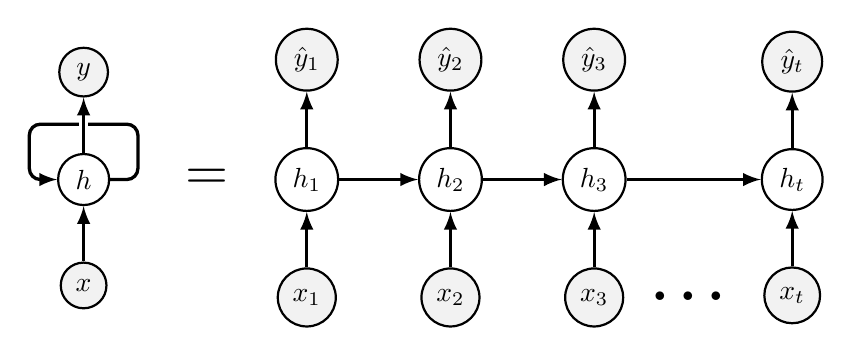
\begin{tikzpicture}[item/.style={circle,draw,thick,align=center},
itemc/.style={item,on chain,join}]
\begin{scope}[start chain=going right,nodes=itemc,every
join/.style={-latex,very thick},local bounding box=chain]
\path node (h1) {$h_1$} node (h2) {$h_2$} node (h3) {$h_3$} node[xshift=2em] (ht)
{$h_t$};
\end{scope}
\node[left=1em of chain,scale=2] (eq) {$=$};
\node[left=2em of eq,item] (AL) {$h$};
\path (AL.west) ++ (-1em,2em) coordinate (aux);
\draw[very thick,-latex,rounded corners] (AL.east) -| ++ (1em,2em) -- (aux) 
|- (AL.west);
\foreach \T in {1,2,3,t} 
{\draw[very thick,-latex] (h\T.north) -- ++ (0,2em)
	node[above,item,fill=gray!10] (y\T) {$\hat y_\T$};
	\draw[very thick,latex-] (h\T.south) -- ++ (0,-2em)
	node[below,item,fill=gray!10] (x\T) {$x_\T$};}
\draw[white,line width=0.8ex] (AL.north) -- ++ (0,1.9em);
\draw[very thick,-latex] (AL.north) -- ++ (0,2em)
node[above,item,fill=gray!10] {$y$};
\draw[very thick,latex-] (AL.south) -- ++ (0,-2em)
node[below,item,fill=gray!10] {$x$};
\path (x3) -- (xt) node[midway,scale=2,font=\bfseries] {\dots};
\end{tikzpicture}
\end{document}
	\caption{Illustration of a RNN. The right hand side shows  the time unfolded structure, which explicitly depends on time.}
	\label{fig:rnn}
\end{figure}

Assume that we have temporarily ordered features $\{x_t\}$ and labels $\{y_t\}$, with  $x_t \in \mathbb R^{d_x}$ and $y_t \in \mathbb R^{d_y}$. There are many formulations of RNNs. One of the simplest RNNs, the Eilman RNN, takes as internal memory state $h_t$ the expression \cite{ELMAN1990179, Goodfellow:2016:DL} 
\begin{align}
	h_t &= \gamma_h\left(W_{h_1} h_{t-1} + W_{h_2} x_t + b_h\right) \\
	y_t &= \gamma_y\left(W_y h_t + b_y\right),
\end{align} 
where $W_{h_1} \in \mathbb R^{d_h \times d_h} ,W_{h_2} \in \mathbb R^{d_h \times d_x}, b_h \in  \mathbb R^{d_h}$ and  $W_y \in \mathbb R^{d_y \times d_h}, b_y \in \mathbb R^{d_y} $. Training corresponds to learning these weights. Together with their usual demand for initialization the initial state is taken as $h_0=0$.
$\gamma_h$ and $\gamma_y$ are activation functions (a common choics is $\gamma_h(\cdot) = \operatorname{thanh} (\cdot)$ and $\gamma_y(\cdot) = \operatorname{softmax} (\cdot)$ for classification). The \textbf{advantages }of  RNN are 
\begin{itemize}
	\item They can process input sequences of any length. As a consequence  RNNs do not require the explicit specification of a lookback window.
	\item The model size is invariant with respect to input size.
	\item The computation for step $t$ in principle uses information from many steps back.
\end{itemize} 
The \textbf{disadvantage} are
\begin{itemize}
	\item Slow computation.
	\item  Very limited temporal memory in practice \cite{bengio_long_term_rnn_1994, 2001_kolen_gradien_flow_rnn}, which is implied by the exploding and vanishing gradient problem. \cite{Goodfellow:2016:DL}.    One can show that the matrix norm of the partial derivatives necessary for back propagation is  of the form $\lVert \partial h_t / \partial h_k \rVert \leq \beta_1 \beta_2 ^ {t-k}$, which can easily explode or vanish for large time differences $t-k$.
\end{itemize}
There are several RNN \textbf{design patterns}, 
\begin{itemize}
	\item RNN that produce at time step an output and have recurrent connections between hidden units. (E.g., decoder part in sequene to sequence models)
	\item RNN that have recurrent connections between hidden units and only produce an output at the final time step. (E.g., encoder part in sequene to sequence models)
	\item \textit{Bi-directional} RNN that use future information for predictions. This can be usesful in NLP tasks. The construction of bi-directional essentially doubles the number of weights and ist straight forward. It constructs forward and backward memory cells and then concatinates them. For the Eilmann RNN e.g., this yields
	\begin{align}
		 \overrightarrow{h}_t &= \gamma_h\left(\overrightarrow{W}_{h_1} \overrightarrow{h}_{t-1} + \overrightarrow{W}_{h_2} x_t + \overrightarrow{b}_h\right) \\
		 \overleftarrow{h}_t &= \gamma_h\left(\overleftarrow{W}_{h_1} \overleftarrow{h}_{t-1} + \overleftarrow{W}_{h_2} x_t + \overleftarrow{b}_h\right) \\
		 h_t  & = \overrightarrow{h}_t \oplus  \overleftarrow{h}_t \\
		y_t &= \gamma_y\left(W_y h_t + b_y\right),
	\end{align}
where $\oplus$ is the direct sum (i.e., concatinate vectors).
\end{itemize}

\paragraph{Long-Short-Term Memory (LSTM)}
LSTMs \cite{lstm, 	schmidhuber_1999_learning_to_forget} try to overcome the limitations in learning long-range dependencies in the data by improving "gradient flow" within the network \cite{Sherstinsky_2020}. This is achieved by a more complex memory state. LSTMs introduce an additional cell state $c_t$,  which stores long-term information with additional temporal modulations conducted by so called gates, 
\begin{align}
	\textit{Input gate:}&  \quad i_t = \sigma \left( 
	 W_{i_1} h_{t-1} + W_{i_2} x_{t} + b_i
	 \right)\\ 
	\textit{Output gate:}& \quad  o_t = \sigma \left( 
	W_{o_1} h_{t-1} + W_{o_2} x_{t} + b_o
	\right)\\ 
	\textit{Forget gate:}& \quad  f_t = \sigma \left(
	W_{f_1} h_{t-1} + W_{f_2} x_{t} + b_f
	 \right), 
\end{align}
where  $W_{i_1}, W_{o_1}, W_{f_1} \in \mathbb{R} ^ {d_h \times d_h}$,  $W_{i_2}, W_{o_2}, W_{f_2} \in \mathbb{R} ^ {d_h \times d_x}$, and $b_i, b_o, b_f \in \mathbb{R}^{d_h}$. $h_t$ is called hidden state and  $\sigma (\cdot)$ is the sigmoid activation function. The gates modify hidden state $h_t$ and cell state $c_t$ at time $t$ according to  
\begin{align}
	 \textit{Cell state}& \quad  c_t = 
	 f_t \odot c_{t-1} + i_t \odot \left (W_{c_1} h_{t-1} + W_{c_2} x_t + b_c  \right) \\
	 \textit{hidden state:}& \quad  h_t = 
	 o_t \odot \tanh(c_{t}), 	 
\end{align}
where $W_{c_1} \in \mathbb{R}^{d_h \times d_h}, W_{c_2} \mathbb{R}^{d_h \times d_x}, b_c \in \mathbb{R}^{d_h}$, and  $\odot$ is the component wise (Hademard) product. The initial states are set to $h_0=c_0=0$.
As with simple RNNs there are many kinds of LSTMs \cite{Greff_2017}, in particular peephole LSTMs \cite{Gers_2001, gers2002learning} and peephole convolutional LSTMs \cite{shi2015convolutional}.

\subsection{Attention mechanism}
The attention mechanism \cite{bahdanau_2016_attention, cho_2014_attention, luong_2015_attention}. Assume a sequence $\{x_1, \dots, x_T\}$ with $x_i \in \mathbb R ^{d_x}$. Then the attention mechanism is of the form
\begin{align}
	x_t' &= \sum_i f(x_i) \, \lambda_{it} \label{eq:attention_context}\\ 
	\lambda_{it} &= \lambda(x_i, x_t) =  \text{softmax}\, g(x_i, x_t) \label{eq:attention},
\end{align}
where  $f$ and $g$ are potentially trainable functions. Different choices for them yield different attention mechanisms. The transformed $x_t'\in \mathbb R ^{d_h}$ is sometimes called context vector or attention. It is common to parametrize the weights $\lambda_{it}$ with the softmax function (\ref{eq:attention}), \footnote{$\text{softmax}\, g(x_i, x_t) = \frac {e^{g(x_i, x_t)} }{\sum_i e^{g(x_i, x_t)}}$}  and call $g$ similarity function. 
\paragraph{Hard vs. soft attention}
The softmax parametrization enables a probabilistic interpretation of the weights $\lambda_{it} = p(i | t)$ with respect to $i$ for a given $t$. The most common approach to obtain a attention function is given in (\ref{eq:attention_context}) as a weighted linear combination over vectors $f(x_i)$. This approach is called \textit{soft attention} and can be directly incorporated with back propagation.

However, one could also sample an $\ell$ of the  $\lambda$-distribution $p(i | t)$  and then use $x_t' = f(x_\ell)$ as attention function instead of averaging (\ref{eq:attention_context}). This approach is called \textit{hard attention} and thus  pays attention only to a specific part of the sequence (for example think of $x_\ell$ as a glimpse of a figure). Hard attention is harder to train as back propagation is not feasible and one has to resort to methods from reinforcement learning.
 
\paragraph{Self Attention}
Self attention computes a transformed $x_t'$ with respect to every element in the sequence $\{x_1, \dots, x_T\}$ - in particular there is also a contribution to (\ref{eq:attention_context}) from $x_t$ it\textit{self}.
Specifically  \cite{vaswani2017attention} parametrizes the  functions $f$ and $g$ with three matrices $W_q,W_k,W_v$, with $W_v \in \mathbb{R}^{d_h \times d_x}$ and $W_q, W_k \in \mathbb{R}^{d_s \times d_x}$. Now, define 
\begin{align}
 q_t := W_q x_t, \quad
 k_i := W_k x_i,  \quad
 v_i :=  W_v x_i,  
 \end{align}
 and identify the functions $f$ and $g$ in  (\ref{eq:attention_context}) - (\ref{eq:attention}) with
 \begin{align}
f(x_i) &:= v_i \\ 
g(x_i, x_t) &:= \frac{k_i ^T q_t}{\sqrt{d_s}} =  \frac{q_t^T  k_i}{\sqrt{d_s}}, 
\end{align}
gives as attention $x'_t = \sum_i v_i \lambda _{it} $
with $\lambda _{it}  = \text{softmax}(q_t^T  k_i/\sqrt{d_s})$. The vectors $v_i  \in \mathbb R^{d_h} $, $q_i\in \mathbb R^{d_s} $ and $k_i \in \mathbb R^{d_s} $ are called value, query and key in analogy with database retrieval systems. 

So for a fixed point in time $t$ the weights are essentially obtained by a scaled dot product of the query vector $q_t$ at $t$ with the key vectors \textit{at all times}  $k_i, i \in \{1, \dots, T\}$ (including $t$ itself). The attention is then the weighted sum over the value vectors $v_i$. 

The formulation can be readily extended to all points in time. Define the matrices 
\begin{align}
X &:=[x_1,\dots, x_T] \in \mathbb{R}^{d_x\times T}\\
Q &:= W_q X \in \mathbb{R} ^ {d_s \times T}, \\ 
K &:= W_k X \in \mathbb{R} ^ {d_s \times T},\\ 
V &:= W_vX\in \mathbb{R} ^ {d_h \times T},
\end{align}
which gives
\begin{align}
	 X' =:\mathcal A (Q, K, V)  = V \lambda, \quad \lambda = \text{softmax}\left(\frac{Q^T K}{\sqrt d_s} \right),
\end{align}
where the softmax function is component wise and the normalization w.r.t to rows. This formulation computes the attention for all times simultaneously ($X':=[x'_1,\dots, x'_T]  \in \mathbb{R}^{d_h\times T}$). Note that in practice rather a dual (i.e., transposed) formulation is used as it is more compatible with sequence conventions (time as leading index).  Either way, \textbf{training corresponds to computing the matrices $W_q,W_k,W_v$} via back propagation.

\paragraph{Multi-head attention}
The idea is to perform self attention in parallel on different subspaces for increased performance. Each individual attention computation within this approach is called \textit{head}. 

Specifically for each  $h$ (\textit{head}) in $1, \dots H$ introduce "projection" - Matrices ${P_{h,q}, P_{h,k},  P_{h,v}}$, where $P_{h,q}, P_{h,k} \in \mathbb{R}^{d_{s'} \times d_s}$ and $P_{h,v} \in \mathbb{R}^{d_{h'} \times d_h}$. Now define

\begin{align}
Q_h &= P_{h,q} W_q X = W_{h,q}  X \in \mathbb{R} ^ {d_{s'} \times T}, \\ 
K_h &= P_{h,k} W_k X = W_{h,k}  X \in \mathbb{R} ^ {d_{s'}  \times T},\\ 
V_h &= P_{h,v} W_vX  = W_{h,v}  X \in \mathbb{R} ^ {d_{h'}  \times T},
\end{align}
and compute the matrix multiplications, which yield effective weight matrices $W_{h,q}, W_{h,k} \in \mathbb{R} ^ {d_{s'} \times d_x}$ and $W_{h,q} \in \mathbb{R} ^ {d_{h'} \times d_x}$.      
The multi-head attention is then the direct sum\footnote{The direct sum is with respect to columns $\mathcal A(Q_i, K_i, V_i)\oplus \mathcal A(Q_j, K_j, V_j) \in \mathbb{R} ^ {2d_{h'}  \times T }$} of the individual attentions together with an additional matrix multiplication by a matrix $W$, 
\begin{align}
	 X' = W\oplus_{h=1}^H \mathcal A(Q_h, K_h, V_h),
\end{align}
where $X' \in \mathbb{R} ^ {H d_{h'}  \times T}$ and $W \in \mathbb{R} ^ {H d_{h'}  \times H d_{h'}}$.
Training corresponds to learning the 3$H$ matrices $\{W_{h,q}, W_{h,k}, W_{h,v}\}$ and the matrix $W$ via back propagation.

\paragraph{Dual formulation} While the the above formulations seem natural if the weight matrices are thought of linear operators in the it is common to use the dual formulation (because conventionally the time index is the first index). This can be achieved by transposing the design matrix $X$ all subsequent expressions and then rename the Matrices. 
So consider matrices of the form $W_v \in \mathbb{R}^{d_x \times d_h}$ and $W_q, W_k \in \mathbb{R}^{d_x \times d_s}$.  Then, in the matrix formulation the attention is given by
\begin{align}
X &:=[x_1,\dots, x_T]^T \in \mathbb{R}^{T\times d_x}\\
Q &:= X W_q \in \mathbb{R} ^ {T \times d_s}, \\ 
K &:= X W_k \in \mathbb{R} ^ {T \times d_s},\\ 
V &:= X W_v \in \mathbb{R} ^ {T \times d_h}, \\ 
X'&=:\mathcal A (Q, K, V)  =  \text{softmax}\left(\frac{Q K^T}{\sqrt d_s} \right) V,
\end{align}
where $\mathcal A (Q, K, V)\in \mathbb{R} ^ {T \times d_h}$ and the element-wise softmax is now normalized with respect to columns. For the multi-head attention choose matrices $P_{h,q}, P_{h,k} \in \mathbb{R}^{d_s \times d_{s'} }$ and $P_{h,v} \in \mathbb{R}^{d_h \times d_{h'} }$ and 
\begin{align}
Q_h &= X W_q  P_{h,q}  = X W_{h,q}   \in \mathbb{R} ^ {T \times d_{s'}}, \\ 
K_h &= X W_k  P_{h,k}  = X W_{h,k} \in \mathbb{R} ^ {T \times d_{s'}},\\ 
V_h &= X W_v P_{h,v}  = X W_{h,v}  \in \mathbb{R} ^ {T\times d_{h'}}, \\
X' &= \oplus_{h=1}^H \mathcal A(Q_h, K_h, V_h) W,
\end{align}
where the direct sum is now with respect to  columns.



\paragraph{Causal attention}
So far there was no notion auf causality. For a given point in time $t$ the attention ranges over the whole time period and thus also w.r.t to future events. In order to introduce temporal causality contributions from future events should vanish in (\ref{eq:attention_context}): $\lambda _{it} = 0$ for $i > t$. In the parametrization of self attention this can be achieved by masking
\begin{align}
\mathcal A (Q, K, V)  =  \text{softmax}\left(\frac{Q K^T}{\sqrt d_s} + M\right) V,	
\end{align}
where $M$ is $-\infty$ in the upper triangular and 0 elsewhere.



\subsection{Sequence to sequence models and transformers}
The problem with RNNs are i) long range dependencies ii) vanishing and exploding gradients, iii) large number of training steps and iv) the recurrence prevents from parallel training. \textit{All} of these problems are improved by transformer networks. 
Transformers are entirely based on attention. They just look at contextual similarity and thus inherently neglect temporal ordering. Therefore the temporal ordering (positions) is incorporated by adding positional encoding to the input features.


\begin{itemize}
	 \item compare methods: https://jalammar.github.io/illustrated-bert/
	 \item http://jalammar.github.io/illustrated-word2vec/
	 \item https://www.youtube.com/watch?v=5vcj8kSwBCY
%	 \item implementation of attention layer https://github.com/tensorflow/models/blob/master/official/nlp/transformer/attention_layer.py
%	 \item https://www.youtube.com/watch?v=8zAP2qWAsKg&list=RDCMUCP7jMXSY2xbc3KCAE0MHQ-A&start_radio=1&rv=8zAP2qWAsKg&t=5337
%	 \item https://www.youtube.com/watch?v=8zAP2qWAsKg&t=2410s
%	 \item implementation: https://colab.research.google.com/github/tensorflow/docs/blob/master/site/en/tutorials/text/nmt_with_attention.ipynb#scrollTo=nZ2rI24i3jFg
	 
\end{itemize}

\section{Normalizing flows}
Baysian methods allow to model uncertainties. While there are methods of its own for Bayesian modeling via a Baysian belief network there are approaches that incorporate these ideas into neural network architectures \cite{bayesion_networks_tutoral_2020}. 

In principle there are two sources for uncertainty. \textbf{Epistemic uncertainty} is inherent to the model due to the likelihood function, which is of the general $p(y  | x, \theta)$ form for a supervised problem for a target random variable $Y$ given covariates $X$ and model parameters $\theta$.  \textbf{Aleotoric uncertainty} is the uncertainty on the model parameters coming from limited training data $D$, $p(\theta | D)$. 

For likelihood functions, and hence epistemic uncertainty the traditional approach is to parametrize the likelihood function by some analytic pdf. In the context of neural networks these parameters are learned by a neural network with suitable activation functions in the output layer to fit the domain of definitions of these parameters. While this allows to incorporate features into the likelihood function in a non-linear fashion this may still limit the expressiveness of the model as it hinges on the particular choice of the likelihood function. In order to overcome this limitation recent attempts aim to learn the likelihood function in a parameter free fashion via normalizing flows \cite{normalizing_flows_2019, normalizing_flow_review_kobyzev_2021}, diffusion models \cite{https://doi.org/10.48550/arxiv.2006.11239}, or implicit quantile regression \cite{pmlr-v80-dabney18a}

\subsection{Transformation of random variables}
Consider two random variables $X, Y \in \mathbb{R}^d$ with probability distributions 
$p_X, p_Y$. Let $f$ be an \textbf{bijective }function such that $f(X) = Y$. Then the two probability distributions are linked by the change of variable formular. 
\begin{align}
p_Y(y) &= p_X(f^{-1}(y)) |\det Df^{-1}(y)| \label{eq:pdf_trafo} 
\end{align}
where $Df^{-1}(y)=\partial f^{-1} / \partial y $ is the Jacobian evaluated at point $y$. The density $p_Y$ is also sometimes called \textit{push forward} of $p_X$ by the function $f$, $f_*p_X$. So, given $f$ and $p_X$  one can compute the pdf $p_Y$. As $f$ is bijective then the inverse transformation is
\begin{align}
	p_X(x) = p_Y(f(x)) |\det Df(x)|. \label{eq:pdf_trafo_inv} 
\end{align}

Now we ask a more complicated question. Let there be given  two probability distributions $p_X, p_Y$ - does there exist a bijective function $f$ that transforms these distributions into each other? However, from a practical point of view the mere existence is not enough as (\ref{eq:pdf_trafo}) dictates that the inverse and the Jacobi determinant should be cheap to compute. \cite{Bogachev_2005, jaini_polynomial_flow_2019}.
Fortunately there is theoretical support,
\begin{definition}{(Triangular map)}
	A map $T=(T_1, \dots, T_d): \mathbb{R}^d  \rightarrow \mathbb{R}^d $ is called triangular if $T_1$ is a function of $x_1$, $T_2$ a function of $(x_1, x_2)$, and so on: $T_i$ is a function of $(x_1,\dots, x_i)$. A triangular map is called (strictly) increasing if every component $T_i$ is (strictly) increasing with respect to the variable $x_i$ (keeping the other variables $(x_1, \dots, x_{i-1})$ fixed).
\end{definition}

\begin{theorem}{\cite{Bogachev_2005, jaini_polynomial_flow_2019}} \label{thm:bogachev}
	For any two densities $p_X$, $p_Y$ over $X=Y=\mathbb{R}^d$ there exists a unique increasing triangular map $T: X \rightarrow Y$ such that $p_Y = T_*p_X$.
\end{theorem}

Consider some properties of triangular maps.
First, the Jacobian of a triangular map is triangular because $\partial T_i /\partial x_j = 0 \text{ for } j > i$ and therefore the Jacobian determinant can be computed from the diagonal elements $\det DT = \prod_i \partial T_i /\partial x_i$. 
The inverse strictly increasing triangular map is also a triangular map.
\begin{align}
	T^{-1} &= (T^{-1}_1, \dots, T^{-1}_d): \mathbb{R}^d  \rightarrow \mathbb{R}^d \label{eq_inv_triang}
\end{align}

Consider the  scalar map  $t_i :x_i \mapsto T_i(x_1, \dots x_i)$, for fixed $x_1, \dots x_{i-1}$. The inverse $t_i^{-1}$ exists because this map is strictly increasing. This establishes the components of $T^{-1}$
\begin{align}
	&T_1^{-1}(y_1) = t_1^{-1}(y_1) \nonumber \\ 
	&T_2^{-1}(y_1,y_2) = t_2^{-1}(T_1^{-1}(y_1),y_2) \nonumber \\
	&\dots \nonumber \\
	&T_d^{-1}(y_1,\dots, y_d) = t_d^{-1}(T_1^{-1}(y_1), \dots, T_{d-1}^{-1}(y_1, \dots,y_{d-1} ), y_d) \label{eq:inv_triang_rec}
\end{align}
Apparently this is a triangular map\footnote{Note that abuse of notation for $d=1$: $t_1^{-1}$ is the inverse of $T_1$. But $T^{-1}_1$ is also denoted as the first component of the inverse map}. We need to show that it is indeed the inverse map $T^{-1}\circ T = T\circ T^{-1} = id$. We show this by induction in $d$. For $d=1$ this is apparently true. Assume that the statment holds fof $d-1$. Pick $x \in \mathbb R^d$, the components of $T(x)$ are given by $y_1 = T_1(x_1), y_2 = T_2(x_1, x_1), \dots y_d = T_d(x_1, \dots, x_d)$. By the induction assumption
we have $T_1^{-1}(y_1)=x_1 \dots, T_{d-1}^{-1}(y_1, \dots y_{d-1})=x_{d-1}$.  For the last component we have $T_d^{-1}(y_1,\dots, y_d) = t_d^{-1}(T_1^{-1}(y_1), \dots, T_{d-1}^{-1}(y_1, \dots,y_{d-1} ), y_d) = t_d^{-1}(x_1, \dots x_{d-1}, y_d)$ for fixed $x_1, \dots x_{d-1}$.  But this is a scalar function and its value at $y_d$ is by construction $x_d$. Thus $T^{-1}\circ T = id$. And similar for $T\circ T^{-1}=id$

From a computational point of view the inverse $T^{-1}$ needs to be computed iteratively as $T^{-1}_i$ relies on $T^{-1}_{1}, \dots, T^{-1}_{i-1}$. Therefore it cannot be computed in a parallel fashion (as opposed to $T$), which can be a limiting factor for models with high dimensions. However, the good news is that each component of this recursion is just the inverse of a scalar function, which can be computed fairly easy also numerically (if necessary).


The composition of triangular maps is again a triangular map. Consider two triangular maps $T$ with $x_i' = T_i(x_1, \dots, x_i)$ and $T'$ then $(T'\circ T)_i = T'_i(x'_1, \dots, x'_i) = T'_i(T_1(x_1), \dots, T_i(x_1, \dots, x_i))$ only depends in $x_1, \dots, x_i$. $T'\circ T$ is (strictly) increasing if $T$ and $T'$ are.

In summary,
\begin{itemize}
	\item The Jacobian of a triangular map is triangular and the Jacobian Determinant can be computed from the diagonal entries only $\det DT = \prod_i \partial T_i /\partial x_i$.
	\item The inverse of  a strictly increasing triangular map is triangular and given by Eqs. (\ref{eq_inv_triang}) and (\ref{eq:inv_triang_rec}).
	\item The composition of triangular maps $T = T^n \circ \dots \circ T^2 \circ T^1 $ is triangular and the Jacobian  factorizes $DT = \prod_{i=1}^{n} DT^i $. If the $T^i$ are strictly increasing then the inverse of $T$  is given by $T = {T^{1}}^{-1} \circ \dots  \circ {T^{n}}^{-1}$. 
\end{itemize}

\paragraph{Todo:} 
\begin{itemize}
\item look at paper again: do we need strictly increasing map $T$ in order to assure invertibility? The paper has outlined this ...
\item Also the general trafo rule \label{eq:pdf_trafo}  requires a bijective function. The paper comes around to this and shows the formular for increasing triangular functions with a one sided derivative.
\item Use examples from \cite{jaini_polynomial_flow_2019} to show that this is not so mystical at all (cdf in 1 d case¸)
 \item conditional version (probably a clean formulation helps with variational autoencoders)
 
\end{itemize}


\subsection{Normalizing Flows: basic idea}
\begin{figure}[h!]
	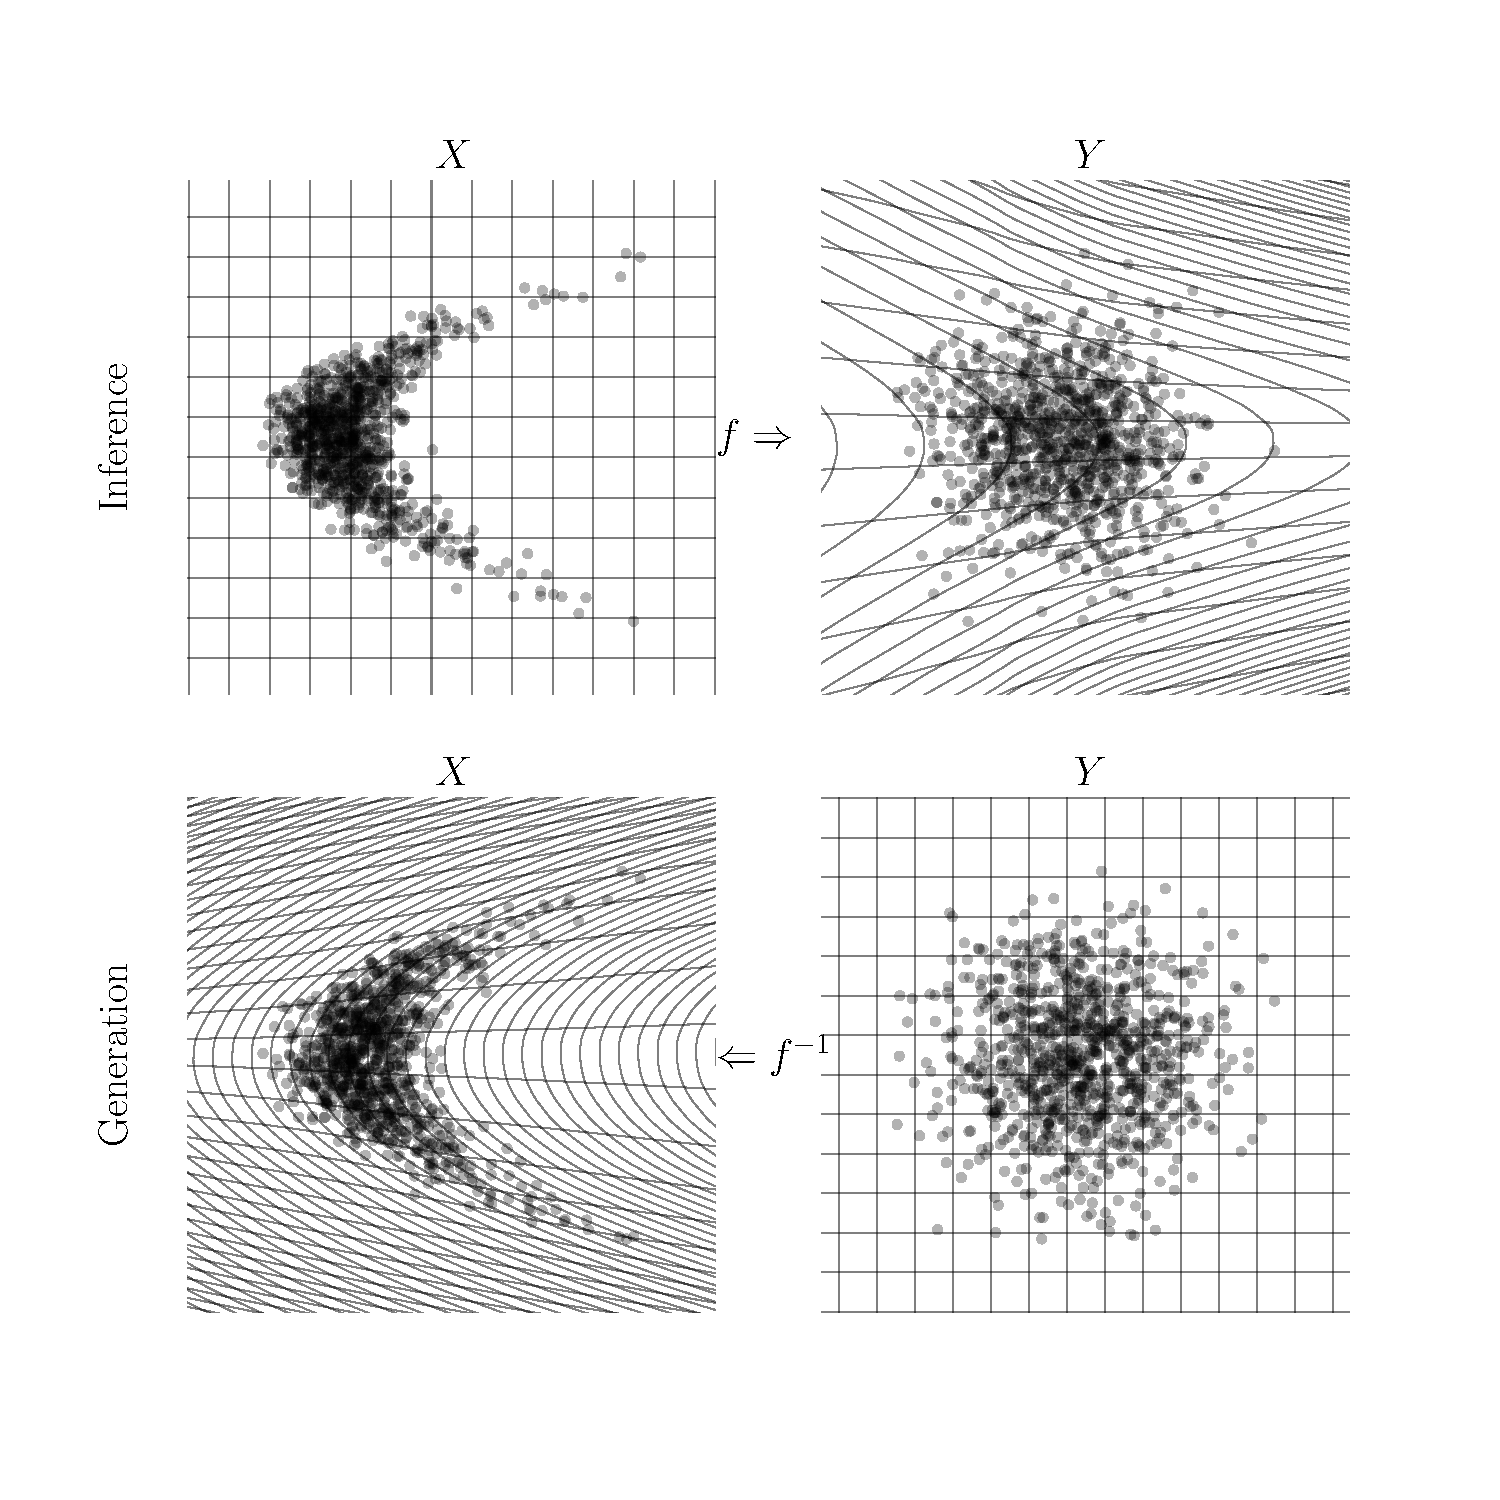
\includegraphics[width=\linewidth]{normalizing_flow_img.pdf}
	\caption{Illustration of normalizing flow.}
	\label{fig:normalizing_flow}
\end{figure}
Let $p_X$ be a complicated distribution and $p_Y$ a known, tractable pdf (uniform or normal distribution). Further assume that we only have samples of $p_X$ $\mathcal D = \{x^{(i)}\}_{i=1}^N$ exists, but is unknown otherwise. We would like to learn a tringular map $f: X\rightarrow Y$ by a neural network  (Fig. \ref{fig:normalizing_flow}).

If we could succeed in learning $f$ then we can use it in two fold manner. We could use it for density estimation and data generation by drawing samples from the known base distribution $y \sim p_Y$ and then obtain new samples in the target distribution $p_X$ from $f^{-1}(y)$. From this samples all relevant statistical properties can be computed.
 Furthermore this approach can be also used to construct flexible test distributions for the approximate posterior in variational inference \cite{rezende_2015}.


Let the base distribution be parametrized by parameters $\phi$, such that $p_Y(y) = p_Y(y|\phi)$ and denote the neural network parameters of $f$ by $\theta$, $f_\theta(x) = f(x|\theta)$. The training (inference) task is to estimate the parameters of the base distribution and the function $\Theta = (\phi,\theta)$ from $\mathcal D$. 

In order to learn the parameters $\theta$ of $f$ one needs to define a loss function, which shall be minimized. This loss function should "compare" the pdfs from the inverse transformation induced by $f$ from (\ref{eq:pdf_trafo_inv}) $p_X(x|\Theta)$ and the true, unknown distribution $p_X(x)$  (of which, we only have samples) in some sense. There are several possible loss functions and the Kullback-Leibler\footnote{$\text{KL}(q||p) = \int q(x) \ln \frac{q(x)}{p(x)} \, dx=  \langle \ln q \rangle_q - \langle \ln p \rangle_q$} divergence is an obvious one:
\begin{align}
\mathcal L (\Theta, \mathcal D) &= \text{KL}(p_X(x) \, || \, p_X(x | \Theta)) \nonumber \\ 
&=  -  \langle \ln p_X(x | \Theta) \rangle _{p_X} + const. \nonumber \\ 
& \approx - \frac{1}{N}\sum_i^N \ln p_X(x^{(i)} | \Theta) + const.  \nonumber \\ 
& = - \frac{1}{N}\sum_i ^N \left\{ \ln p_Y(f(x^{(i)} | \theta)\, |\, \phi) + \ln |\det Df(x^{(i)}|\theta)|  \right\}+ const., \label{eq:nf_kl}
\end{align}
where the constant terms are contributions independent of the paramters to optimize ($\Theta=\{\theta, \phi\}$). In the second line the expectation value w.r.t. the unknown exact pdf is approximated by the empirical mean (Monte-Carlo approximation) given samples from $\mathcal D$. So (\ref{eq:nf_kl}) can be used to determine gradients on the function $\partial_\theta \mathcal L (\Theta)$ and on the base distribution $\partial_\phi \mathcal L (\Theta)$ needed to minimize the Kullback-Leibler divergence. Note however, that in some implementations only the parameters of $f$ are learned keeping the base distribution fixed.


 Alternatively we could aim to determine the parameters $\Theta$ in order maximize the log-likelihood, $\ln p_X(\mathcal D | \Theta)$, and thus minimize the negative of it, 
\begin{align}
\mathcal L (\Theta,\mathcal D) &= - \ln p_X(\mathcal D| \Theta) \nonumber \\ 
&=  - \ln \prod _{i=1}^N p_X(x^{(i)}| \Theta) \nonumber \\
&= - \sum_i ^N \left\{ \ln p_Y(f(x^{(i)} | \theta)\, |\, \phi) + \ln |\det Df(x^{(i)}|\theta)|  \right\},
\label{eq:nf_mll}
\end{align} 
which eventually gives up to the constant $1/N$ the same  gradients as the KL divergence. Therefore, both versions share the same minimizer\footnote{However, when using an optimizer with given step length the optimal step length could be different as the computed gradients differ by $1/N$. 
On the other hand it ist most common to optimize the average of the log likelihood, which gives the same result as the KL approach.}.
There are several other possible loss functions like the Wasserstein metric as reviewed in \cite{normalizing_flows_2019}. 

This is summarized in the basic normalizing flow algorithm for inference and data generation in algorithms \ref{algo:normalizing_flow_inference} and  \ref{algo:normalizing_flow_generation}, respectively. 

\begin{algorithm}[t] \label{algo:normalizing_flow_inference}
\SetAlgoLined
\textbf{Input:} \\ 
\quad Data $\mathcal D $ \\
\quad A base distribution $p_Y(\cdot|\phi)$ \\
\quad A function $f_\theta$ \\
\KwResult{Learned parameters $\phi, \theta$}
\textbf{Initialize:} $\phi, \theta$ \\
\While{SGD not converged}{
	$\mathcal M \sim \mathcal D¸$ (Random minibatch of data) \\
	Compute loss $\mathcal L (\theta, \phi, \mathcal M)$ from Eq. (\ref{eq:nf_kl}) \\
	Compute gradients $\partial_\theta \mathcal L(\theta, \phi, \mathcal M)$, 
	$\partial_\phi \mathcal L(\theta, \phi, \mathcal M)$ \\
	Udate $\theta, \phi$ using SGD optimizer
}
\caption{Inference of a normalizing flow model using stochastic gradient descent (SGD)}
\end{algorithm} 

\begin{algorithm}[t] \label{algo:normalizing_flow_generation}
	\SetAlgoLined
	\textbf{Input:} \\ 
	\quad A base distribution $p_Y(\cdot|\phi)$ \\
	\quad A function $f_\theta$ \\
	\KwResult{Sample $x \sim p_X(\cdot | \theta)$}
	{
	$y \sim p_Y(\cdot|\phi)$  \\
	$x = f^{-1}_\theta(y)$
}
	\caption{Data generation with a normalizing flow}
\end{algorithm} 
\subsection{Constructing $f$}
So far no statement of how to construct $f$ has been made. Theorem \ref{thm:bogachev} suggests to construct $f$ as a triangular map. The theorem only guarantees that there is an increasing triangular map. However, as we wish to generate samples from the inverse map in practice strictly increasing triangular maps are constructed. Surprisingly some of these have been shown to be universal \cite{jaini_polynomial_flow_2019, huang_2018_neural_autoregressive_flows}.



\section{Variational Autoencoders}
\cite{Kingma_2019_AnIntroductionToVariationalAutoencoders}


\section{Time Series Neural Networks}
Common practices for time series modelling
\begin{itemize}
	\item \textbf{Split time} in context and prediction times
	\item \textbf{Scaling:} scale data over context time and rescale after prediction
	\item \textbf{Metrics for evaluation} \textit{Continuous Ranked Probability Score} (CRPS) for probabilistic time series models
	\item \textbf{Dequantization:} corresponds to adding noise (e.g. from a uniform distribution) for disrecte data when using models that require contineous data (eg. normalizing flow models).
	\item \textbf{Categorical features:} use embeddings 
\end{itemize}
Time series can be understood as subclass of sequence models. This section summarizes explicit time series models.
\paragraph{LSTNet.} This network \cite{lstnet_2017} aims to model long and short term patterns by combining neural net components with an autoregressive model. A prediction at time step $t$ given by

\begin{align}
	\hat y_t = y_t^{AR} + y_t^{NN},
\end{align}
where $y_t^{NN}$ is the  neural net component and $y_t^{AR}$ is the auto regressive component. The auto regressive part is sensitive to the scale of the inputs (which is a hard for neural networks). This significantly improves model performance. 

The neural network part models modulations with respect to this baseline model. It introduces a so called recurrent skip connection by adapting the formulae of e.g. LSTM (in the paper of GRU): LSTM  uses hidden states at time $t-1$ as inputs for time $t$. The paper instead uses hidden states of time step $t-p$ as input for time step $t$. This adds a parameter $p$ (the number of hidden states skipped through) and needs to be tuned. For periodic patterns $p$ is obviously the periodicity. This method should increase the long term capacity of standard RNNs.
\begin{align}
 	\text{Temporal convolution: } y_t \mapsto y'_t \\
 	\text{Gated recurrent network: } y'_t \mapsto y''_t \\ 
	\text{Recurrent-skip network: } y'_t \mapsto y'''_t \\ 	
	\text{Combination } y_t^{NN} = W^1y''_t +  \sum_{i=0}^{p-1}W^2_iy'''_{t-i} + b   
\end{align}
The convolution shall capture short term dependencies and serves as input for following RNN. The RNN should capture long term time dependencies and even more the recurrent skip network.  Finally both recurrent units are combined by a small dense NN. As input serve only the last hidden state at time $t$ of the RNN (context vector) and the last $p$ hidden states of the recurrent-skip network. Instead of the last two steps also the attention mechanism can be used (which also increases the long term capacity). The authors find similar accuracy within these two approaches.


\section{Outlook}
\begin{itemize}\setlength\itemsep{0em}
\item Practical tips \cite{2012arXiv1206.5533B, Hinton2012Practical, DBLP:series/lncs/7700} 
\item Interpretation of NN \cite{2017arXiv170607979M, KinSchAlbMueErhKimDae18}
\item (Denoising) autoencoder 
\item Adversarial nets (generative vs. discriminative)
\item Hopfield networks \cite{ramsauer2020hopfield}
\item Convolution neural networks 
\item Hyper parameter tunining using Gaussian processes
\item eg VGG http://www.robots.ox.ac.uk/~vgg/practicals/cnn/index.html
\end{itemize}

\appendix
\section{Numerics}
\paragraph{Log-sum-exponent trick.} The logarithm of sum of exponentials may suffer from numerical overflow (due to exponent) or underflow. A numerical stable equivalent is
\begin{align} \label{log-sum-exp-trick}
	\ln \sum_i e^{x_i}  =  \ln \sum_i e^{x_i - c} + c, \quad c = \max\{x_i\}, 
\end{align}
which prevents the exponent to explode (numerical overflow). This idea may be put forward compute numerical stable logarithms of matrix multiplication. 
More generally, consider the logarithm of a Tensor contraction  
\begin{align}
\ln \sum_k A_{ikl} B_{ikl} &= \ln \sum_k e^{\ln A_{ikl}} e^{\ln B_{ikl}} \\
& = \ln \sum_k \exp({\ln A_{ikl} + \ln B_{ikl}}) 
\end{align}
As a special case the matrix product is given by
\begin{align}
\ln A B_{ij} = \ln \sum_k A_{ik} B_{kj} = \ln \sum_k \exp({\ln A_{ik} + \ln B_{kj}}),  
\end{align}
both can be computed in a numerical stable fashion using (\ref{log-sum-exp-trick}). Furthermore the logarithm of a Matrix product can be written as a generalized sum of the individual Matrix logarithms.


\bibliographystyle{plain}
\bibliography{paper}
\end{document}